% GNUPLOT: LaTeX picture with Postscript
\begingroup
  \makeatletter
  \providecommand\color[2][]{%
    \GenericError{(gnuplot) \space\space\space\@spaces}{%
      Package color not loaded in conjunction with
      terminal option `colourtext'%
    }{See the gnuplot documentation for explanation.%
    }{Either use 'blacktext' in gnuplot or load the package
      color.sty in LaTeX.}%
    \renewcommand\color[2][]{}%
  }%
  \providecommand\includegraphics[2][]{%
    \GenericError{(gnuplot) \space\space\space\@spaces}{%
      Package graphicx or graphics not loaded%
    }{See the gnuplot documentation for explanation.%
    }{The gnuplot epslatex terminal needs graphicx.sty or graphics.sty.}%
    \renewcommand\includegraphics[2][]{}%
  }%
  \providecommand\rotatebox[2]{#2}%
  \@ifundefined{ifGPcolor}{%
    \newif\ifGPcolor
    \GPcolortrue
  }{}%
  \@ifundefined{ifGPblacktext}{%
    \newif\ifGPblacktext
    \GPblacktextfalse
  }{}%
  % define a \g@addto@macro without @ in the name:
  \let\gplgaddtomacro\g@addto@macro
  % define empty templates for all commands taking text:
  \gdef\gplbacktext{}%
  \gdef\gplfronttext{}%
  \makeatother
  \ifGPblacktext
    % no textcolor at all
    \def\colorrgb#1{}%
    \def\colorgray#1{}%
  \else
    % gray or color?
    \ifGPcolor
      \def\colorrgb#1{\color[rgb]{#1}}%
      \def\colorgray#1{\color[gray]{#1}}%
      \expandafter\def\csname LTw\endcsname{\color{white}}%
      \expandafter\def\csname LTb\endcsname{\color{black}}%
      \expandafter\def\csname LTa\endcsname{\color{black}}%
      \expandafter\def\csname LT0\endcsname{\color[rgb]{1,0,0}}%
      \expandafter\def\csname LT1\endcsname{\color[rgb]{0,1,0}}%
      \expandafter\def\csname LT2\endcsname{\color[rgb]{0,0,1}}%
      \expandafter\def\csname LT3\endcsname{\color[rgb]{1,0,1}}%
      \expandafter\def\csname LT4\endcsname{\color[rgb]{0,1,1}}%
      \expandafter\def\csname LT5\endcsname{\color[rgb]{1,1,0}}%
      \expandafter\def\csname LT6\endcsname{\color[rgb]{0,0,0}}%
      \expandafter\def\csname LT7\endcsname{\color[rgb]{1,0.3,0}}%
      \expandafter\def\csname LT8\endcsname{\color[rgb]{0.5,0.5,0.5}}%
    \else
      % gray
      \def\colorrgb#1{\color{black}}%
      \def\colorgray#1{\color[gray]{#1}}%
      \expandafter\def\csname LTw\endcsname{\color{white}}%
      \expandafter\def\csname LTb\endcsname{\color{black}}%
      \expandafter\def\csname LTa\endcsname{\color{black}}%
      \expandafter\def\csname LT0\endcsname{\color{black}}%
      \expandafter\def\csname LT1\endcsname{\color{black}}%
      \expandafter\def\csname LT2\endcsname{\color{black}}%
      \expandafter\def\csname LT3\endcsname{\color{black}}%
      \expandafter\def\csname LT4\endcsname{\color{black}}%
      \expandafter\def\csname LT5\endcsname{\color{black}}%
      \expandafter\def\csname LT6\endcsname{\color{black}}%
      \expandafter\def\csname LT7\endcsname{\color{black}}%
      \expandafter\def\csname LT8\endcsname{\color{black}}%
    \fi
  \fi
  \setlength{\unitlength}{0.0500bp}%
  \begin{picture}(7370.00,5102.00)%
    \gplgaddtomacro\gplbacktext{%
      \csname LTb\endcsname%
      \put(1078,704){\makebox(0,0)[r]{\strut{}$0$}}%
      \csname LTb\endcsname%
      \put(1078,1294){\makebox(0,0)[r]{\strut{}$10000$}}%
      \csname LTb\endcsname%
      \put(1078,1885){\makebox(0,0)[r]{\strut{}$20000$}}%
      \csname LTb\endcsname%
      \put(1078,2475){\makebox(0,0)[r]{\strut{}$30000$}}%
      \csname LTb\endcsname%
      \put(1078,3066){\makebox(0,0)[r]{\strut{}$40000$}}%
      \csname LTb\endcsname%
      \put(1078,3656){\makebox(0,0)[r]{\strut{}$50000$}}%
      \csname LTb\endcsname%
      \put(1078,4247){\makebox(0,0)[r]{\strut{}$60000$}}%
      \csname LTb\endcsname%
      \put(1078,4837){\makebox(0,0)[r]{\strut{}$70000$}}%
      \csname LTb\endcsname%
      \put(1210,484){\makebox(0,0){\strut{}$0$}}%
      \csname LTb\endcsname%
      \put(2033,484){\makebox(0,0){\strut{}$0.02$}}%
      \csname LTb\endcsname%
      \put(2857,484){\makebox(0,0){\strut{}$0.04$}}%
      \csname LTb\endcsname%
      \put(3680,484){\makebox(0,0){\strut{}$0.06$}}%
      \csname LTb\endcsname%
      \put(4503,484){\makebox(0,0){\strut{}$0.08$}}%
      \csname LTb\endcsname%
      \put(5326,484){\makebox(0,0){\strut{}$0.1$}}%
      \csname LTb\endcsname%
      \put(6150,484){\makebox(0,0){\strut{}$0.12$}}%
      \csname LTb\endcsname%
      \put(6973,484){\makebox(0,0){\strut{}$0.14$}}%
      \put(176,2770){\rotatebox{-270}{\makebox(0,0){\strut{}Liczba zliczeń J}}}%
      \put(4091,154){\makebox(0,0){\strut{}Gęstość wodoru w próbce wzorcowej $\rho_H $ [g/cm$^3$]}}%
    }%
    \gplgaddtomacro\gplfronttext{%
      \csname LTb\endcsname%
      \put(5986,4664){\makebox(0,0)[r]{\strut{}$ J = 430112 \rho _H  + 9487,86 $}}%
    }%
    \gplbacktext
    \put(0,0){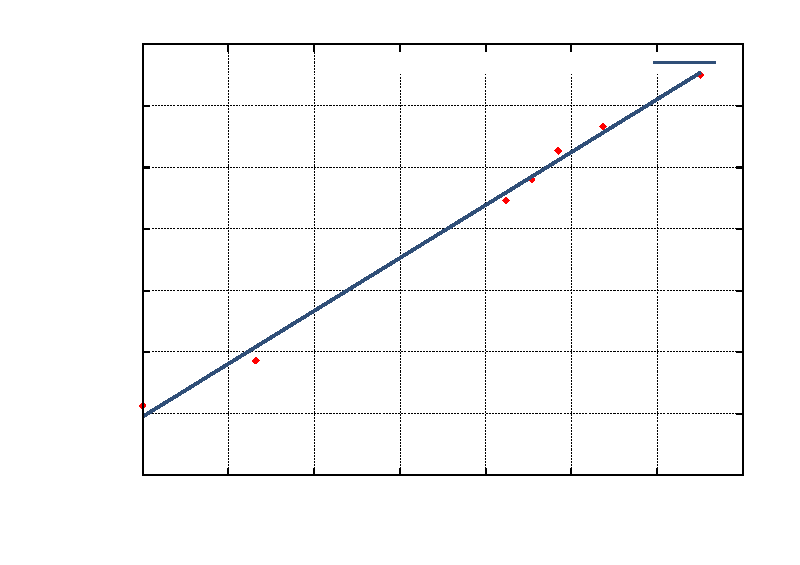
\includegraphics{cechowanie}}%
    \gplfronttext
  \end{picture}%
\endgroup
